\makeatletter\def\input@path{{theme/}}\makeatother
\documentclass{UnBeamer}

\usepackage[brazilian]{babel}
\usepackage[utf8]{inputenc}
\usepackage[T1]{fontenc}
\usepackage{lmodern}
\usepackage{csquotes}
\graphicspath{{figuras/}}

\usepackage[backend=biber, style=numeric]{biblatex}
\addbibresource{referencias.bib}
\setbeamertemplate{bibliography item}[text]
\AtBeginBibliography{\footnotesize}

% Caixa reservando espaço para figuras/capturas de tela ainda não incluídas.
\newcommand{\placeholder}[2][.8\textwidth]{%
     \fbox{\parbox[c][.4\textheight][c]{\dimexpr#1-2\fboxsep-2\fboxrule}{\centering\color{gray}#2}}%
}


\makeatletter
\renewcommand{\unbeamerrightfooter}{%
    \usebeamerfont{author in head/foot}%
    \insertframenumber/\inserttotalframenumber\hspace*{\unbeamer@halfMarginWidth}%
}
\makeatother

%% ------------ Identificação ------------ %%
\title[Eye-tracking para Acessibilidade]{Aplicativo de acessibilidade com uso de eye-tracking}
\author[Medeiros \& Rabelo]{%
    Miguel C. de Medeiros \and Thiago C. R. Rabelo\\[1ex]
    {\small Orientador: Prof. Dr. Edson Mintsu -- ENE/UnB}%
}
\institute[CIC/UnB]{%
    Departamento de Ciência da Computação\\
    Universidade de Brasília\\
    Curso de Engenharia de Computação%
}
\date{}

\begin{document}

\frame{\titlepage}

%% ============================================================ %%
\section{Introdução}

\subsection{Problemas Enfrentados}
\begin{frame}
    % BUSCAR UMA FONTE QUE CONFIRME TUDO ISSO
    \framesubtitle{Esclerose Lateral Amiotrófica (ELA)}
    \begin{itemize}
        \item \textbf{O que é}
        \begin{itemize}
            \item Doença neurodegenerativa progressiva dos neurônios motores~\cite{ela}
            \item Fraqueza e paralisia gradual dos músculos voluntários
        \end{itemize}
        \vfill
        \item \textbf{Impacto na comunicação}
        \begin{itemize}
            \item A fala se deteriora até ser perdida
            \item Mãos e braços também perdem movimento: escrever e digitar
                  deixam de ser opção
            \item A cognição costuma ser preservada: a pessoa continua tendo
                  o que dizer
        \end{itemize}
        \vfill
        \item \textbf{Movimento ocular preservado}
        \begin{itemize}
            \item Os músculos dos olhos costumam ser poupados até fases avançadas
            \item O olhar se torna o principal canal de comunicação
        \end{itemize}
    \end{itemize}
\end{frame}

\subsection{Soluções Existentes}
\begin{frame}
    \small
    \begin{columns}[T]
        \column{.48\textwidth}
            \begin{block}{Smartbox~\cite{smartbox}}
                \begin{itemize}
                    \item Câmera infravermelha Lumin-i acoplada ao tablet
                    \item Tolera movimentos da cabeça e luz do sol
                    \item Grid 3: símbolos, teclado com predição e voz
                \end{itemize}
            \end{block}
            \centering
            \placeholder{Solução existente}
        \column{.48\textwidth}
            \centering
            \placeholder{Solução existente}
            \begin{block}{Tobii Dynavox~\cite{tobii}}
                \begin{itemize}
                    \item Sensor infravermelho embutido (reflexo na córnea e pupila)
                    \item Tela traseira mostra o texto ao interlocutor
                    \item TD Snap e Communicator 5 para comunicação
                \end{itemize}
            \end{block}
    \end{columns}
    % \centering
    % \placeholder{Solução existente}
\end{frame}

\begin{frame}
    \small
    \begin{exampleblock}{O que oferecem}
        \begin{itemize}
            \item Rastreamento preciso, mesmo sob luz do sol
                  e com movimentos da cabeça
            \item Comunicação completa: símbolos, teclado com
                  predição e voz
            \item Controle do ambiente
            \item Aparelho resistente, para cadeira de rodas ou cama
        \end{itemize}
    \end{exampleblock}
    \begin{alertblock}{Mas a que custo?}
        \begin{itemize}
            \item Exigem câmera infravermelha e tablet dedicados
            \item Grid Pad 13 com Lumin-i: US\$~16.485~\cite{smartboxprecos}
            \item TD I-13: US\$~15.565~\cite{tobiipreco}
            \item Fora do alcance da maioria das famílias, ainda
                  sem impostos de importação
        \end{itemize}
    \end{alertblock}
\end{frame}

\subsection{Nosso Objetivo}
\begin{frame}
    \centering
    \placeholder{Tablet comum}
    \begin{exampleblock}{Objetivo}
        Sistema de rastreamento ocular com sistema de teclado com predição e voz que possa ser utilizado em aparelhos tablet comuns.
    \end{exampleblock}
\end{frame}

%% ============================================================ %%
\section{Tecnologias Utilizadas}

\subsection{Eye-tracking}
\subsubsection{Abordagem}
\begin{frame}
    \centering
    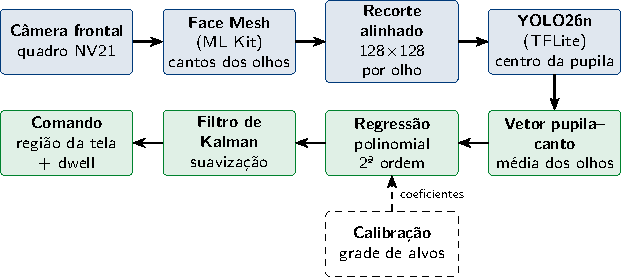
\includegraphics[width=\textwidth, height=.8\textheight, keepaspectratio]{pipeline}
\end{frame}

\subsubsection{Rosto e Olhos: ML Kit Face Mesh}
\begin{frame}
    \small
    \begin{columns}[T]
        \column{.48\textwidth}
            {\normalsize\textbf{ML Kit Face Mesh~\cite{mlkit}}}
                \begin{itemize}
                    \item SDK de aprendizado de máquina do Google para celulares,
                          com inferência no próprio aparelho
                    \item Face Mesh: 468 pontos 3D do rosto em tempo real
                \end{itemize}
        \column{.48\textwidth}
            \centering
            \placeholder[\textwidth]{Rosto com a malha do Face Mesh e os cantos dos olhos destacados}
    \end{columns}
    \begin{exampleblock}{No sistema}
            \begin{itemize}
                \item Localiza o rosto e os cantos de cada olho
                \item Os cantos definem o recorte do olho e a referência do vetor pupila--canto
                \item Não marca a pupila: daí o segundo modelo
            \end{itemize}
    \end{exampleblock}
\end{frame}

\subsubsection{Pupila: YOLO}
\begin{frame}
    \small
    \setbeamerfont{block title}{size=\small}
    \begin{block}{YOLO26n~\cite{yolo,yolo26}}
        Detector de objetos que prevê as caixas numa única passada da rede. \\
        Versão nano da Ultralytics, voltada a dispositivos sem GPU.
    \end{block}
    \begin{columns}[T]
        \column{.48\textwidth}
            {\textbf{MPIIGaze~\cite{mpiigaze}}}
            \begin{itemize}
                \item 213.659 imagens de 15 participantes, capturadas pela
                      webcam no uso diário do notebook
                \item 10.654 imagens com o centro da pupila anotado à mão
            \end{itemize}
        \column{.48\textwidth}
            {\textbf{Treinamento}}
            \begin{itemize}
                \item A partir dos pesos pré-treinados do YOLO26n
                \item 21.308 recortes de olho de 128$\times$128~px,
                      com a mesma geometria do app
                \item Separação por participante: 11 no treino,
                      2 na validação, 2 no teste
            \end{itemize}
    \end{columns}
    \begin{exampleblock}{Teste em participantes nunca vistos} Pupila encontrada em 100\% dos 2.332 recortes, com erro mediano de 4,5\% da largura do olho (2,6~px num quadro de 1280$\times$720).
    \end{exampleblock}
\end{frame}

\subsubsection{Regressão}
% SERIA LEGAL PEGAR REFERÊNCIA
\begin{frame}
    % \scriptsize
    % \setbeamerfont{block title}{size=\small}
    \begin{block}{Entrada: vetor pupila--canto}
        \[
            \mathbf{v} = \frac{\mathbf{p} - \frac{1}{2}(\mathbf{c}_A + \mathbf{c}_B)}{\lVert \mathbf{c}_B - \mathbf{c}_A \rVert}
        \]
        $\mathbf{p}$: centro da pupila;\quad
        $\mathbf{c}_A, \mathbf{c}_B$: cantos do olho.
        Média dos dois olhos $\Rightarrow (v_x, v_y)$.
        Invariante a escala e translação: compensa parte do movimento da cabeça.
    \end{block}
    \begin{block}{Modelo: polinômio de 2ª ordem}
        \[
            x_{\text{tela}} = a_0 + a_1 v_x + a_2 v_y + a_3 v_x^2 + a_4 v_y^2 + a_5 v_x v_y
        \]
        Mesma forma para $y_{\text{tela}}$: 6 coeficientes por eixo.
        Saída em fração da tela, de 0 a 1.
    \end{block}
\end{frame}

\subsubsection{Calibragem}
\begin{frame}
    \centering
    \begin{exampleblock}{Ajuste na calibração}
        \begin{itemize}
            \item Grade de $5 \times 5$ alvos: mediana de $\mathbf{v}$ em cada alvo
            \item Mínimos quadrados com regularização ridge, resolvido por
                  eliminação de Gauss
            \item Descarta até 2 alvos mal fixados, enquanto o erro mediano diminuir
        \end{itemize}
    \end{exampleblock}
    % \placeholder{Captura da tela de calibragem}
    \begin{figure}
        \centering
        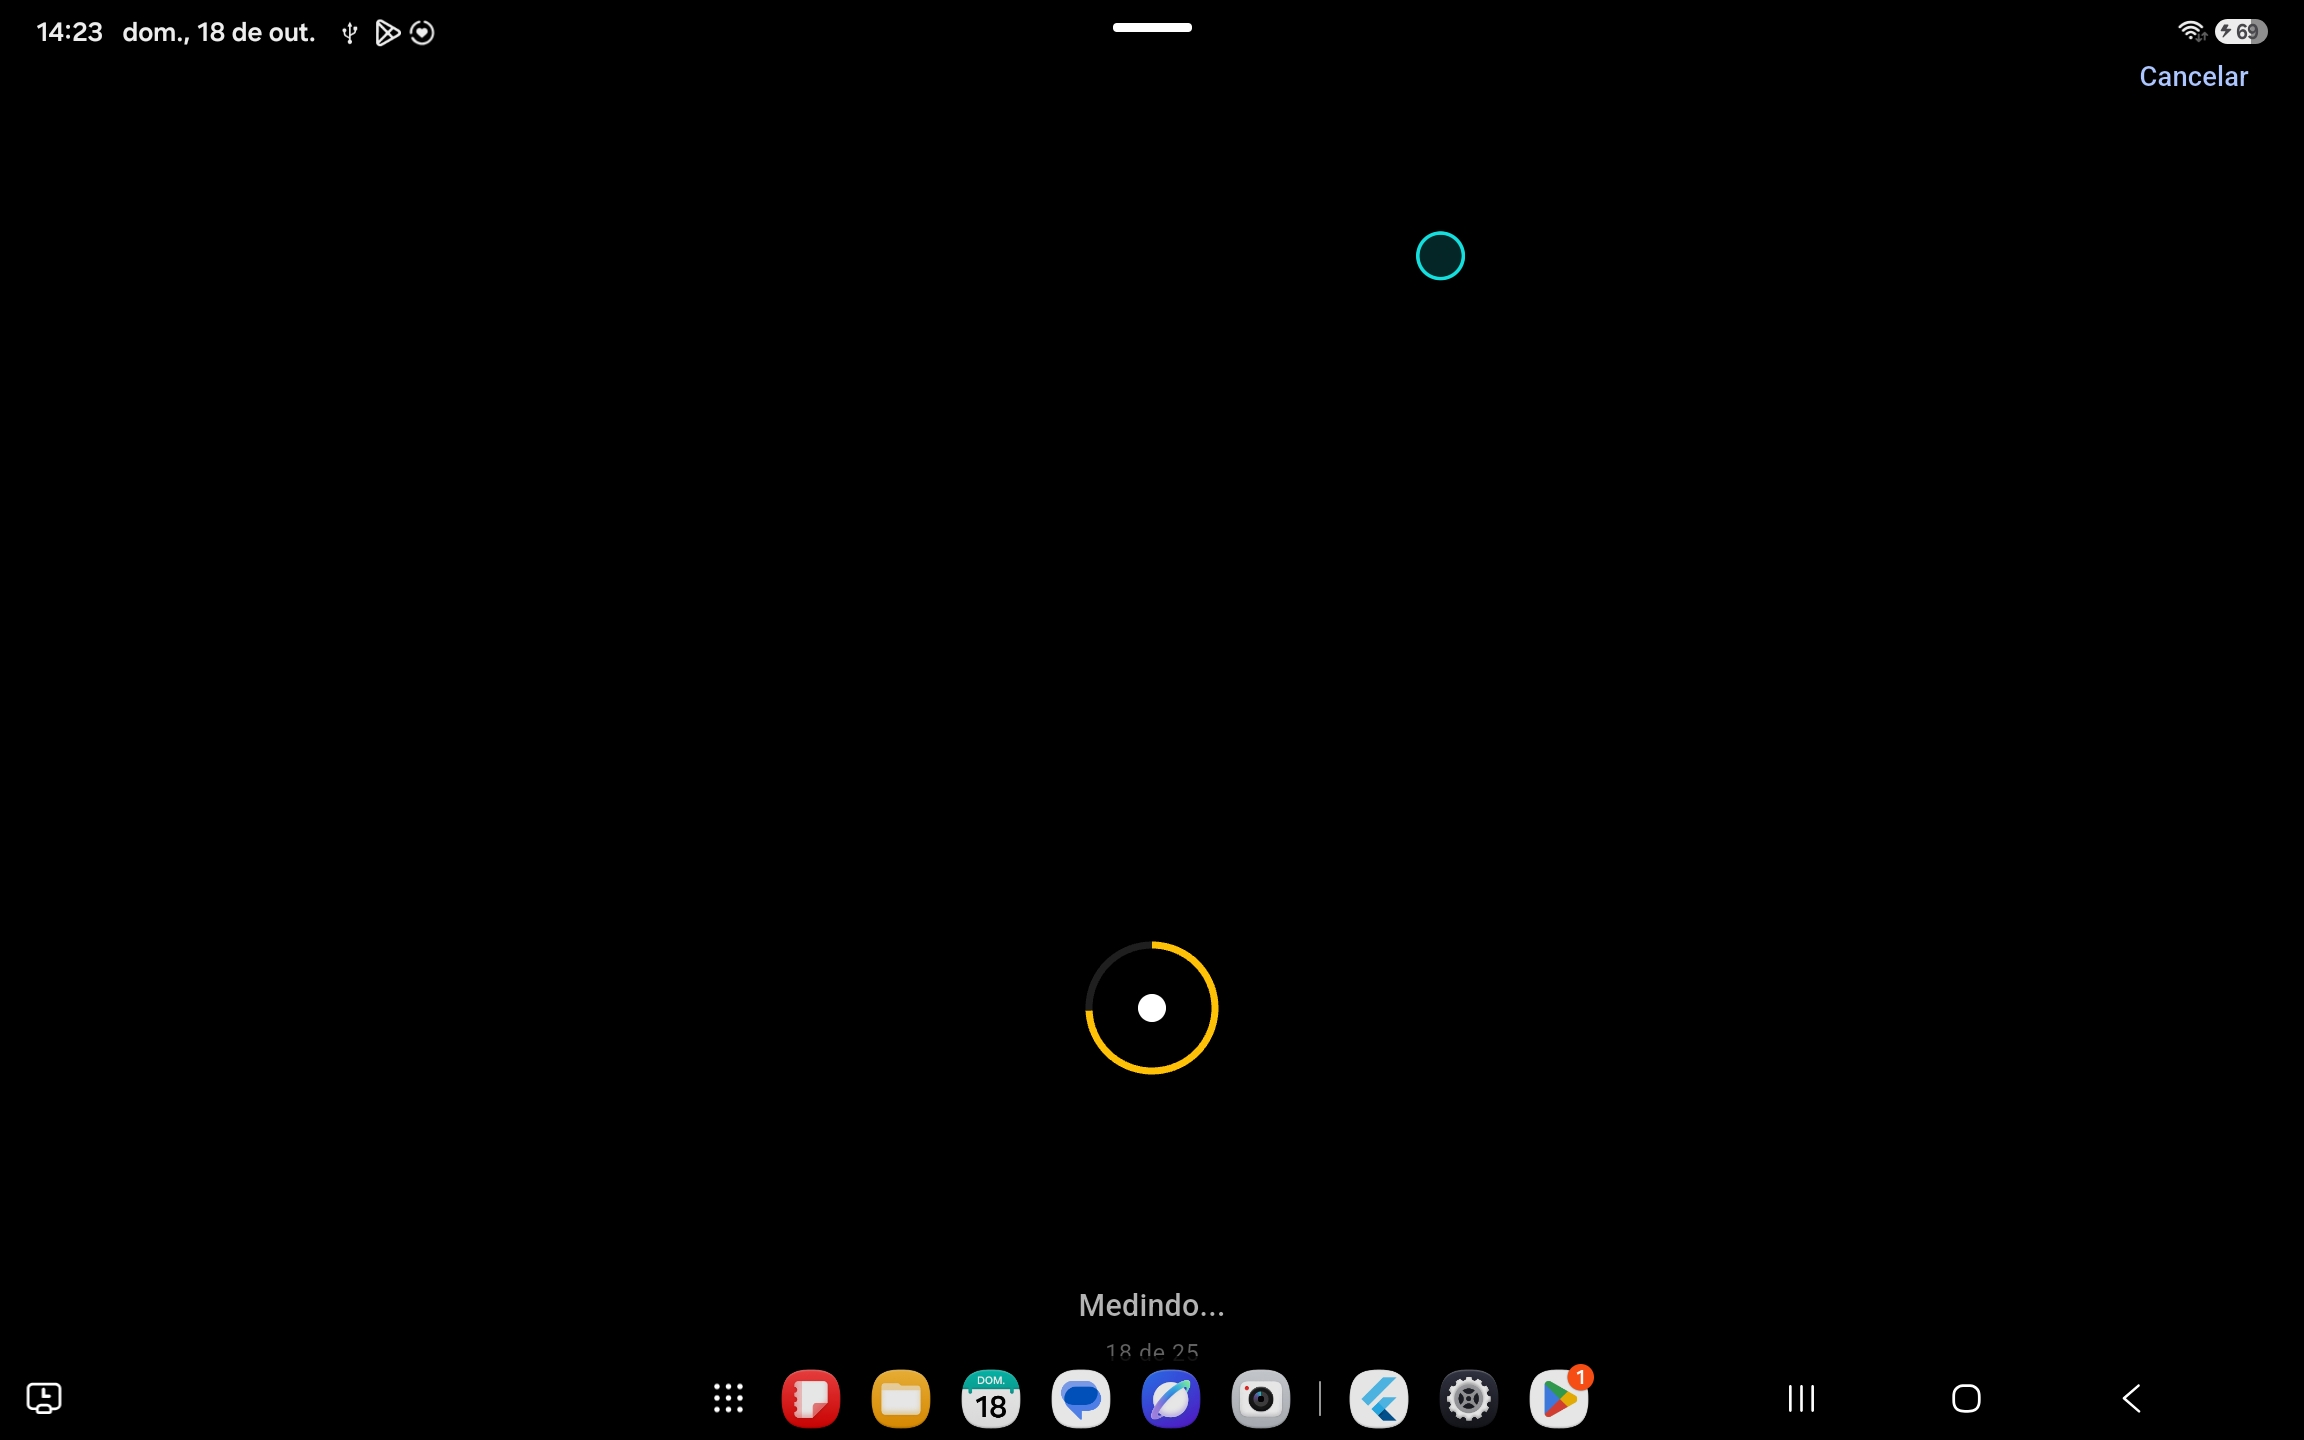
\includegraphics[width=0.6\linewidth]{figuras/tela_calibragem.jpeg}
        % \caption{Caption}
        % \label{fig:placeholder}
    \end{figure}
\end{frame}

\subsubsection{Filtro de Kalman}
\begin{frame}
    \scriptsize
    \setbeamerfont{block title}{size=\small}
    \begin{columns}[T]
        \column{.44\textwidth}
            \begin{alertblock}{Motivação}
                \begin{itemize}
                    \item O ponto da regressão treme a cada quadro: ruído na
                          pupila e nos cantos do olho
                    \item O dwell exige 1,5~s na mesma região: o tremor
                          reinicia a contagem
                \end{itemize}
            \end{alertblock}
            \begin{exampleblock}{No sistema}
                \begin{itemize}
                    \item Um filtro por eixo, $x$ e $y$ independentes
                    \item Variância da medida $R = 0{,}075$ e da
                          aceleração $\sigma_a^2 = 1$
                    \item $\Delta t$ real entre quadros, limitado a 250~ms
                    \item Reiniciado a cada nova calibração
                \end{itemize}
            \end{exampleblock}
        \column{.52\textwidth}
            \begin{block}{Modelo de velocidade constante~\cite{kalman}}
                Estado $\mathbf{x} = (\text{posição}, \text{velocidade})$;
                a aceleração entra como ruído.
                \vspace{-1ex}
                \begin{align*}
                    \text{Predição:}\quad
                    & \hat{\mathbf{x}}^- = F\hat{\mathbf{x}}, \qquad
                      F = \begin{pmatrix} 1 & \Delta t \\ 0 & 1 \end{pmatrix} \\
                    & P^- = F P F^\top + Q \\[1ex]
                    \text{Correção:}\quad
                    & K = \frac{P^- H^\top}{H P^- H^\top + R}, \qquad
                      H = \begin{pmatrix} 1 & 0 \end{pmatrix} \\
                    & \hat{\mathbf{x}} = \hat{\mathbf{x}}^- + K\,(z - H\hat{\mathbf{x}}^-) \\
                    & P = (I - K H)\,P^-
                \end{align*}
                $z$: ponto medido pela regressão.
                O ganho $K$ pondera a previsão e a medida conforme a
                incerteza de cada uma.
            \end{block}
    \end{columns}
\end{frame}


\subsection{Autocomplete}
\subsubsection{Abordagem}
\begin{frame}
    \small
    \begin{figure}
        \centering
        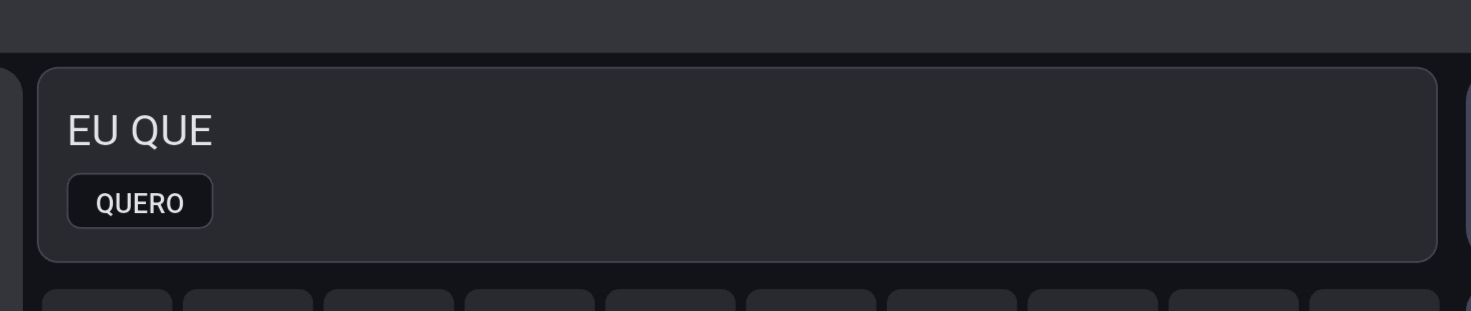
\includegraphics[width=\textwidth]{figuras/tela_teclado_zoom.jpeg}
    \end{figure}
    \begin{columns}[T]
        \column{.52\textwidth}
            \begin{block}{Do texto às sugestões}
                \begin{enumerate}
                    \item Normaliza: minúsculas, sem acento
                    \item Separa as palavras anteriores da
                          palavra em digitação
                    \item Pontua o vocabulário com trigramas
                    \item Mostra as 3 melhores, com acento
                \end{enumerate}
            \end{block}
        \column{.44\textwidth}
            \begin{exampleblock}{Seleção pelo olhar}
                Da primeira linha do teclado, olhar para cima
                entra na barra de sugestões
            \end{exampleblock}
    \end{columns}
\end{frame}

\subsubsection{Modelo de Linguagem: n-gramas}
\begin{frame}
    \small
    \begin{columns}[T]
        \column{.48\textwidth}
            \textbf{Corpus}
            \begin{itemize}
                \item 565 frases típicas de comunicação alternativa,
                      cerca de 765 palavras
                \item Marcador de início de frase: ``eu'' no começo é
                      um contexto diferente de ``eu'' no meio
            \end{itemize}
        \column{.48\textwidth}
            \textbf{Trigramas}
            \begin{itemize}
                \item Conta cada palavra depois das 2 anteriores
                \item Contexto nunca visto: recua para 1 palavra e
                      depois para nenhuma
            \end{itemize}
    \end{columns}
    \begin{block}{Stupid Backoff~\cite{brants}}
        \[
            S(w \mid h) =
            \begin{cases}
                \dfrac{c(h\,w)}{c(h)} & \text{se } c(h\,w) > 0 \\[1.5ex]
                0{,}4 \cdot S(w \mid h') & \text{caso contrário}
            \end{cases}
        \]
        $h$: palavras anteriores;\quad $h'$: $h$ sem a mais antiga;\quad
        $c$: contagem no corpus.
        Não é uma probabilidade, mas basta para ordenar as sugestões.
    \end{block}
\end{frame}

\subsubsection{Completar ou Sugerir a Próxima Palavra}
\begin{frame}
    \small
    \begin{columns}[T]
        \column{.58\textwidth}
            \begin{itemize}
                \item \textbf{Termina em espaço:} sugere a próxima\\
                      \texttt{EU QUERO\textvisiblespace} $\to$
                      BEBER $\cdot$ COMER $\cdot$ IR
                \vfill
                \item \textbf{Palavra pela metade:} completa\\
                      \texttt{EU QUERO B} $\to$
                      BEBER $\cdot$ BOCA $\cdot$ BANHEIRO
                \vfill
                \item \textbf{Ambíguo:} \texttt{E} é a palavra ``e''
                      ou o começo de ``estou''?
            \end{itemize}
        \column{.38\textwidth}
            \centering
            \placeholder[\textwidth]{Barra com \texttt{E} $\to$ ESTOU $\cdot$ EU $\cdot$ A}
    \end{columns}
    \begin{exampleblock}{As duas leituras competem}
        Completar: $S(c \mid h)$
        \qquad
        Próxima palavra: $S(\text{e} \mid h) \cdot S(n \mid h\ \text{e})$\\[1ex]
        \texttt{E} $\to$ ESTOU $\cdot$ EU (completam) $\cdot$ A (vem depois)
    \end{exampleblock}
\end{frame}

\subsubsection{Tolerância a Erros de Digitação}
\begin{frame}
    \small
    \begin{columns}[T]
        \column{.50\textwidth}
            \begin{alertblock}{Problema}
                Uma seta a mais ou a menos troca a letra pela vizinha:
                \texttt{BWB} em vez de \texttt{BEB}, e nenhuma palavra
                começa assim
            \end{alertblock}
            \begin{block}{Distância de edição~\cite{levenshtein}}
                \begin{itemize}
                    \item Até o \emph{prefixo} mais próximo
                    \item Vizinha, letra a mais ou a menos: 1;
                          tecla distante: 2
                    \item Até 1 erro, a partir de 3 letras
                    \item Pontuação $\times\,0{,}01$: as exatas
                          vêm primeiro
                \end{itemize}
            \end{block}
        \column{.46\textwidth}
            \centering
            \placeholder[\textwidth]{Barra com \texttt{EU QUERO BWB} $\to$ BEBER}
    \end{columns}
\end{frame}

\subsubsection{Avaliação Offline}
\begin{frame}
    \small
    \begin{block}{Método}
        \begin{itemize}
            \item Digitador simulado escreve as frases do corpus pelo
                  caminho mínimo de setas e aceita a sugestão quando
                  ela custa menos comandos
            \item Validação cruzada em 10 partes: o modelo nunca viu
                  a frase testada
            \item Mesmas métricas das sessões com pessoas~\cite{soukoreff}
        \end{itemize}
    \end{block}
    \begin{columns}[T]
        \column{.48\textwidth}
            \centering
            \textbf{Sem erros de digitação}\\[1ex]
            \begin{tabular}{lr}
                \hline
                Comandos poupados   & 50,7\% \\
                Palavras entre as 3 & 78,9\% \\
                Fora do vocabulário & 16,5\% \\
                \hline
            \end{tabular}
        \column{.48\textwidth}
            \centering
            \textbf{10\% de letras erradas}\textsuperscript{*}\\[1ex]
            \begin{tabular}{lr}
                \hline
                Sem tolerância & 30,6\% \\
                Com tolerância & 36,6\% \\
                \hline
            \end{tabular}
    \end{columns}
    \vspace{1ex}
    \hfill{\scriptsize * comandos poupados; erro notado só no fim da palavra}
\end{frame}

\subsection{Geração de Áudio}
\begin{frame}
    \begin{itemize}
        \item Kokoro
        \item Sherpa
    \end{itemize}
\end{frame}

%% ============================================================ %%
\section{Desenvolvimento e Arquitetura}

\subsection{Stack}
\begin{frame}
    \begin{itemize}
        \item Flutter \cite{flutter_docs}
        \item Android
        \item Setup e IDE
    \end{itemize}
\end{frame}

\subsection{Módulos}
\begin{frame}
    \centering
     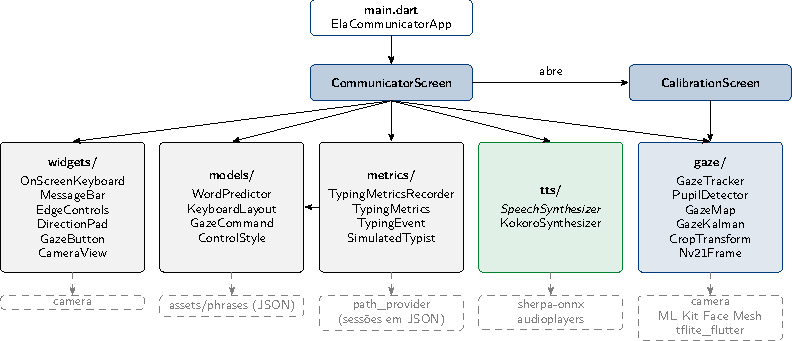
\includegraphics[width=\textwidth, height=.8\textheight, keepaspectratio]{modulos}
\end{frame}

\begin{frame}
    \framesubtitle{Principais Interfaces}
    \scriptsize
        \begin{block}{GazeCommand}
            \texttt{up, down, left, right, select}\\[2pt]
            Contrato único de entrada: olhar, toque e botões
            chegam todos em \texttt{\_handleCommand}.
        \end{block}
        \begin{block}{GazeTracker}
            \texttt{Stream<GazeCommand> commands}\\
            \texttt{Stream<GazeSample> samples}\\
            \texttt{GazeMap? map}\\[2pt]
            Emite um comando quando o dwell completa.
        \end{block}
\end{frame}

\begin{frame}
    \framesubtitle{Principais Interfaces}
    \scriptsize
        \begin{block}{SpeechSynthesizer}
            \texttt{initialize()}, \texttt{speak(text)}, \texttt{stop()}\\
            \texttt{ValueListenable<State> state}\\[2pt]
            Isola a tela do runtime de síntese: Kokoro no app,
            implementação falsa nos testes.
        \end{block}
        \begin{block}{WordPredictor}
            \texttt{List<String> suggest(text, limit: 3)}\\
            \texttt{String accept(text, suggestion)}\\[2pt]
            Trigramas com Stupid Backoff e tolerância a erros;
            \texttt{accept} insere a sugestão na mensagem.
        \end{block}
\end{frame}

%% ============================================================ %%
\section{Resultados}

\subsection{Telas}
\begin{frame}
    \centering
    % \placeholder[.5\textwidth]{Tela 1}\hfill
    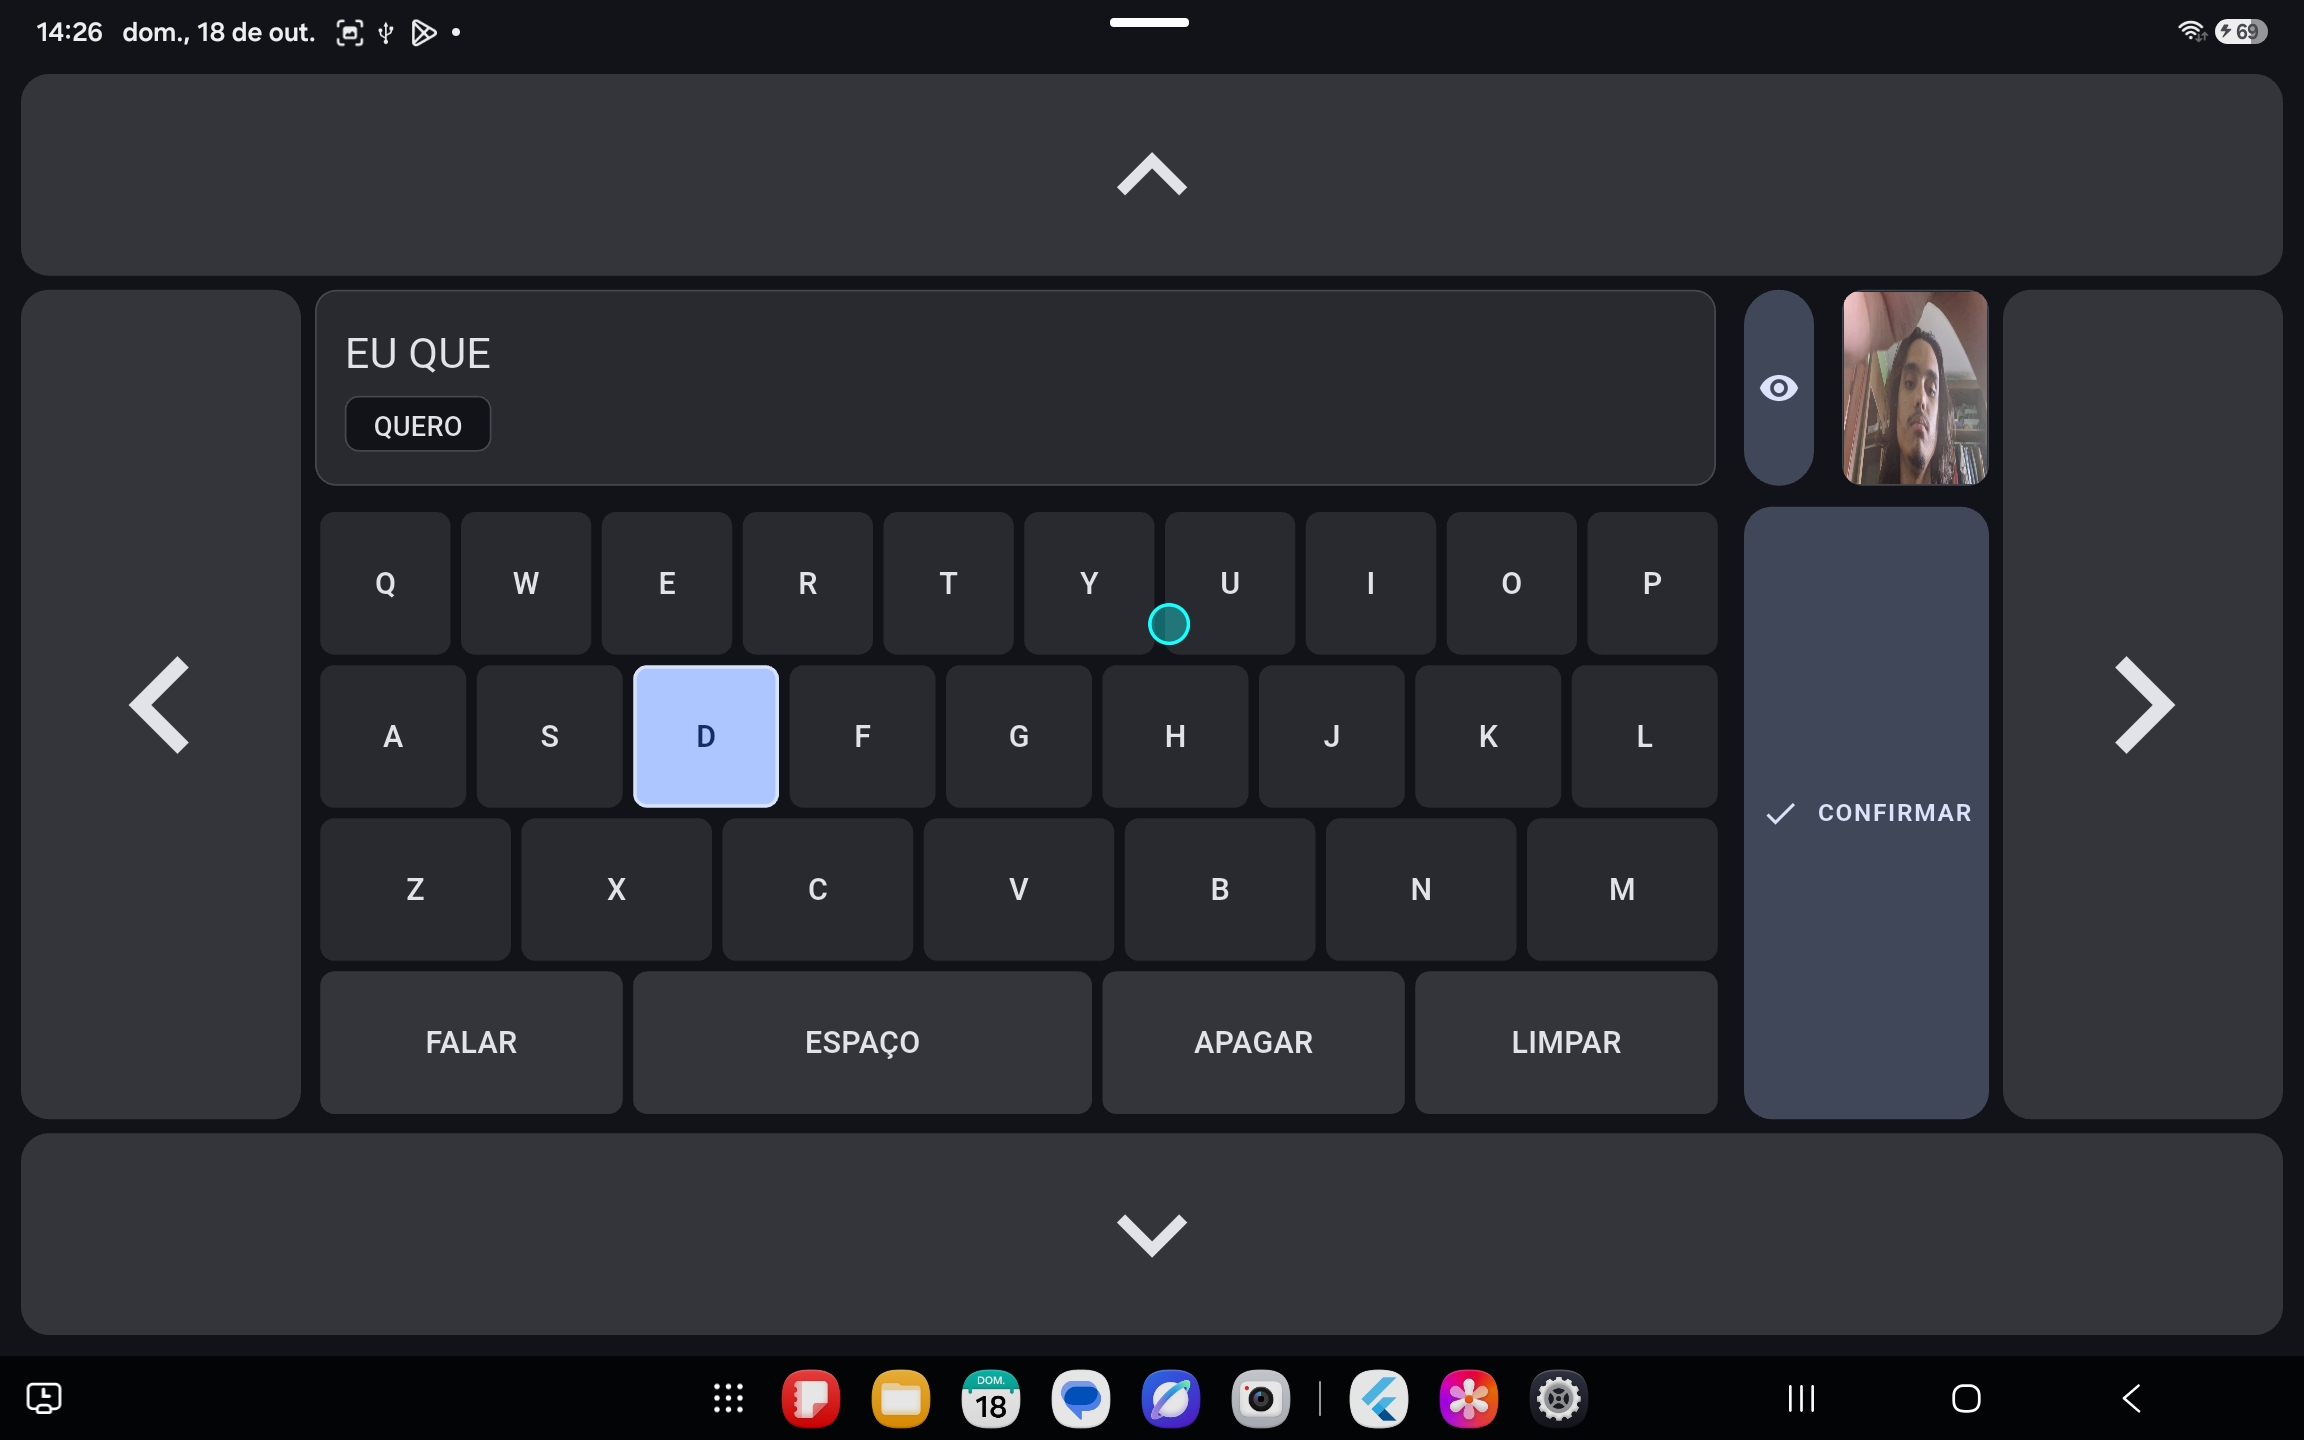
\includegraphics[width=.49\textwidth]{figuras/tela_teclado.jpeg} \hfill
    % \placeholder[.5\textwidth]{Tela 2}
    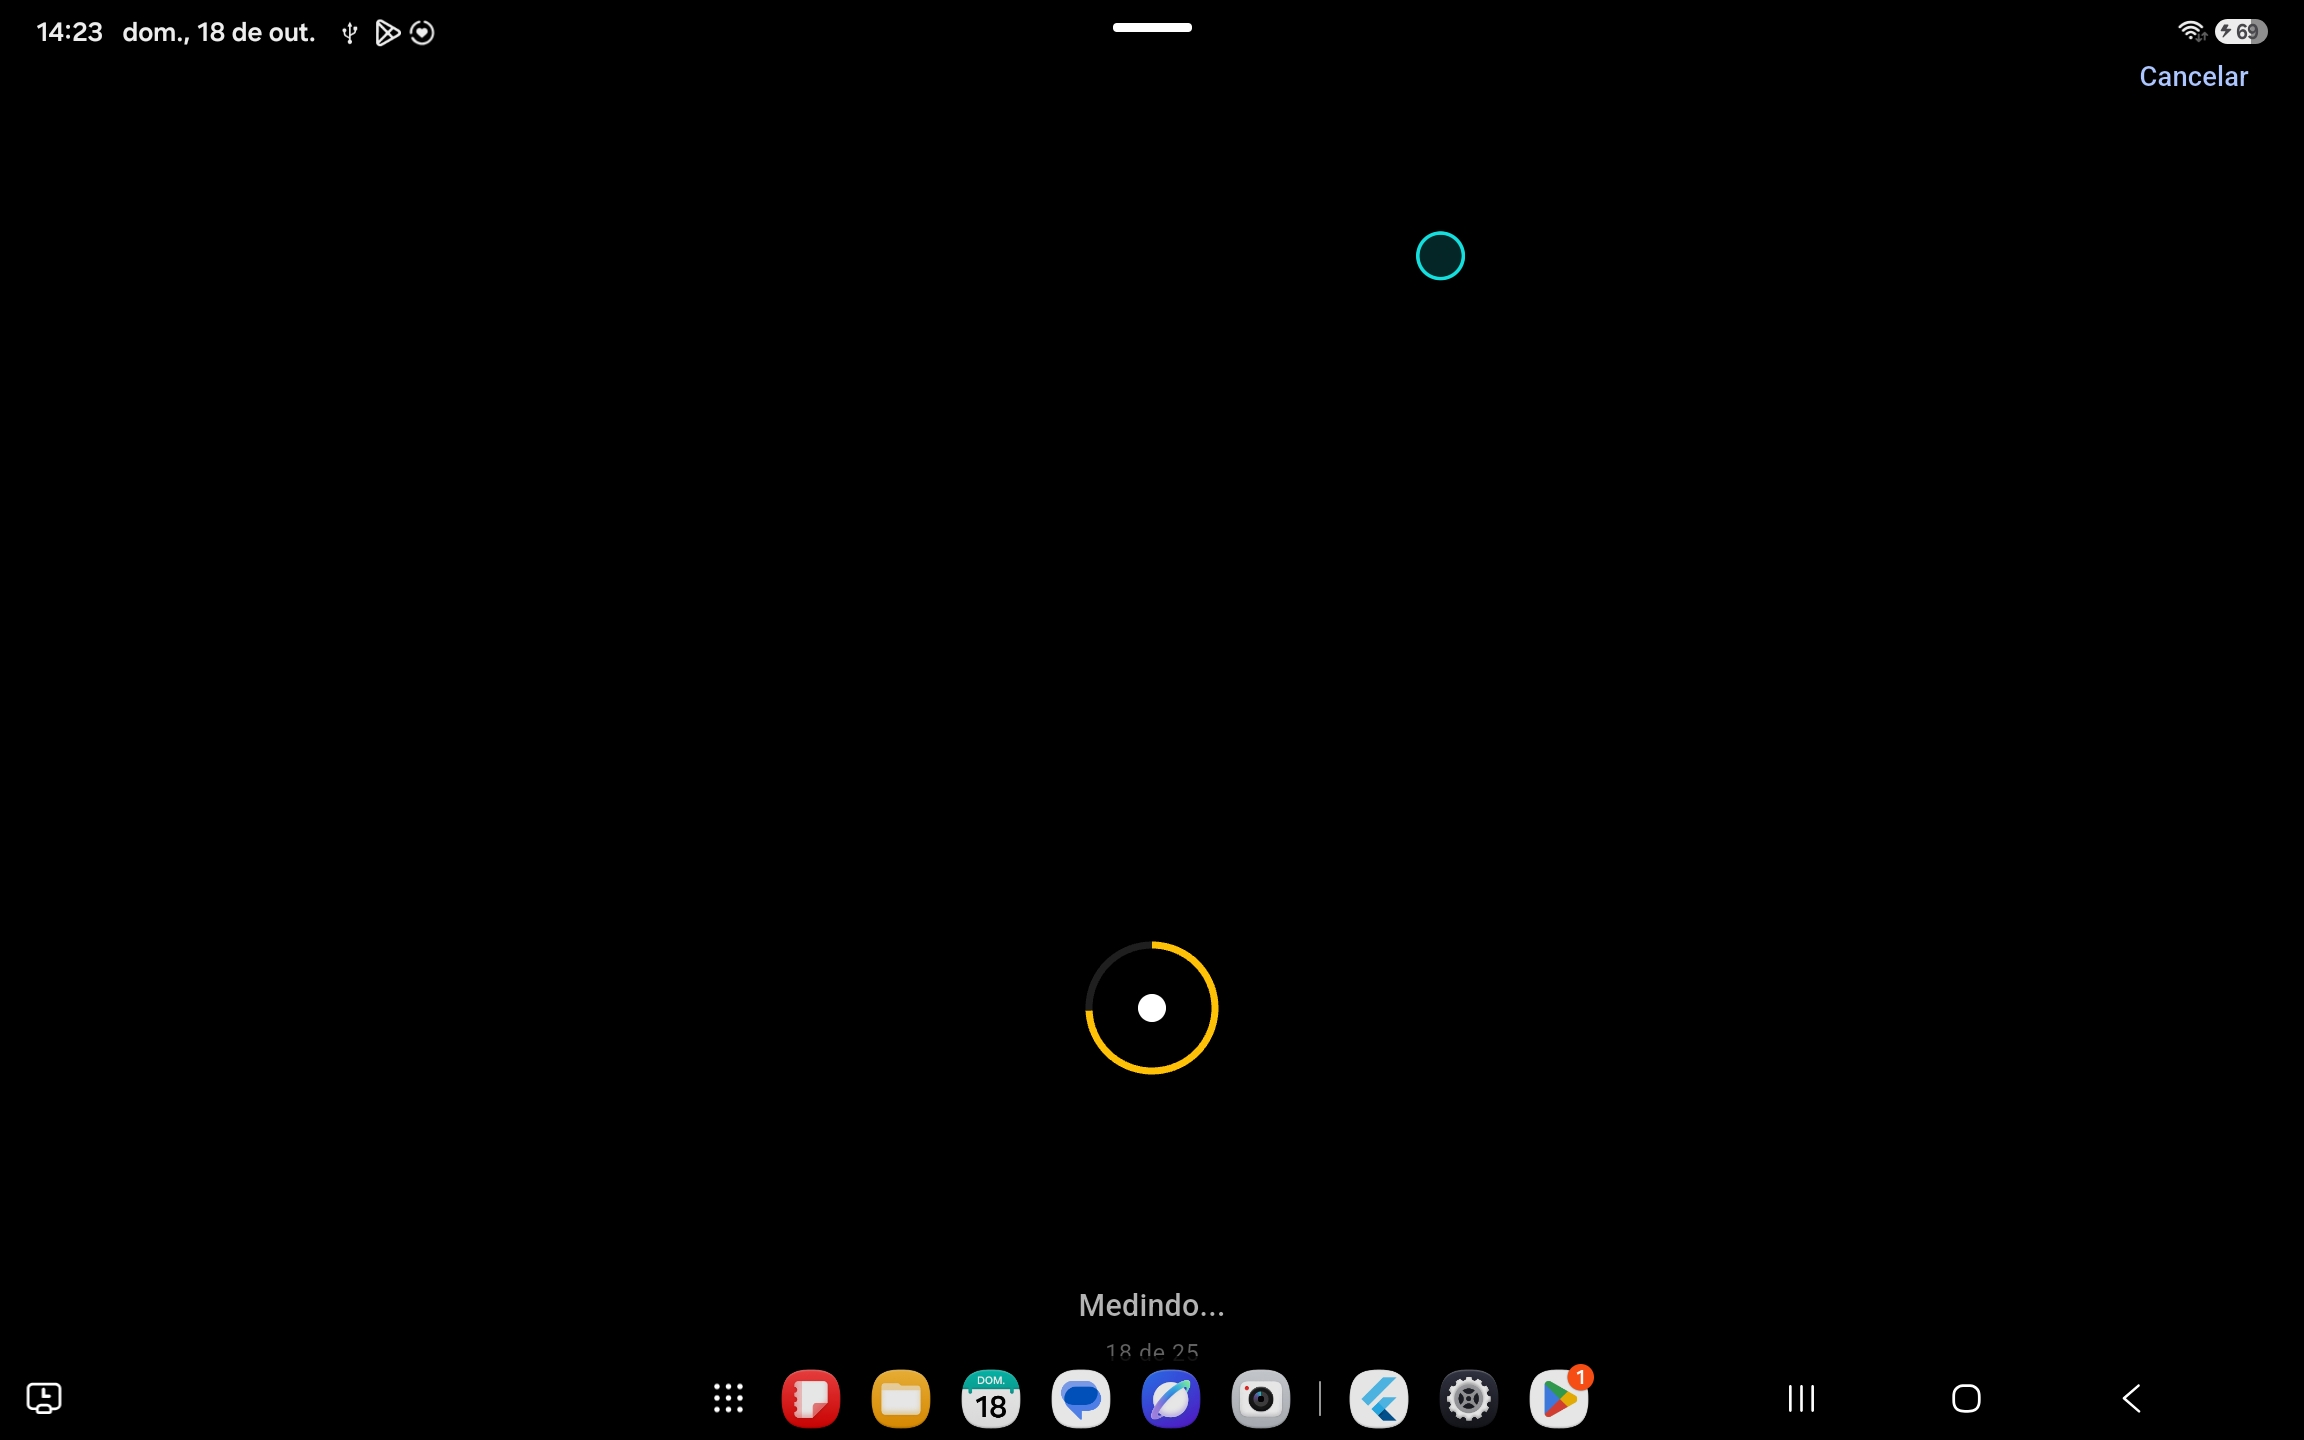
\includegraphics[width=.49\textwidth]{figuras/tela_calibragem.jpeg}
\end{frame}

\subsection{Fluxo de Uso do App}
\begin{frame}
    \centering
    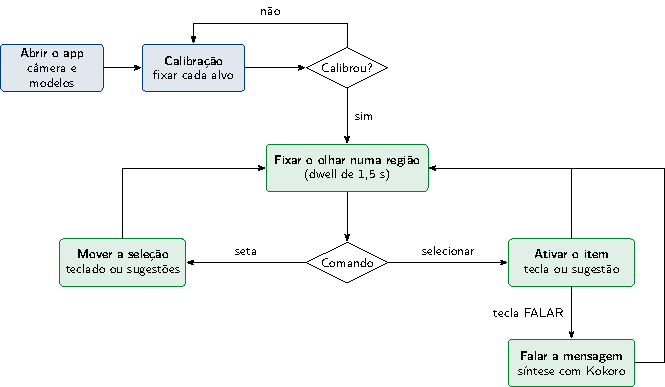
\includegraphics[width=\textwidth, height=.8\textheight, keepaspectratio]{fluxo}
\end{frame}

\subsection{Métricas Obtidas com Pessoas}
\begin{frame}
    \begin{itemize}
        \item Metodologia dos testes
        \item Participantes
    \end{itemize}
\end{frame}

\begin{frame}
    \placeholder{Gráfico/tabela de métricas}
\end{frame}

%% ============================================================ %%
\section{Conclusão}

\begin{frame}
    \begin{itemize}
        \item Síntese dos resultados
    \end{itemize}
\end{frame}

\subsection{Trabalhos Futuros}
\begin{frame}
    \begin{itemize}
        \item Melhoria 1
        \item Melhoria 2
    \end{itemize}
\end{frame}

\section{Referências}

\begin{frame}[allowframebreaks]
    % \nocite{*}
    \printbibliography[heading=none]
\end{frame}

\subsection{Agradecimentos e Perguntas}
\begin{frame}
    \centering\Huge
    \begin{block}{}
        \centering
        Obrigado!\\[2ex]
    \end{block}
    \Large {\color{greenUnB} Perguntas?}
\end{frame}

\end{document}
